\documentclass[12pt]{article}
\usepackage{ucs}
\usepackage[utf8x]{inputenc}
\usepackage[T1]{fontenc}
\usepackage{lmodern}
\usepackage[english]{babel}
\usepackage[nottoc]{tocbibind}
\usepackage[left=2.5cm,right=2.5cm,top=2.5cm,bottom=2.5cm,]{geometry}
\usepackage{graphicx}
\usepackage{nameref}
\usepackage[hidelinks]{hyperref}
\usepackage{sidecap}
\usepackage{wrapfig}
\usepackage[bottom,hang]{footmisc}
\usepackage{acronym}
\usepackage{multirow}
\usepackage{color}
\usepackage{float}

\usepackage{capt-of}
\usepackage{array,				%better tables
			tabularx,			%instead of tabular*
			booktabs,			%tables for good publications
}
\usepackage{afterpage,hyperref}
\usepackage{listings}
\lstset{
    basicstyle=\ttfamily\footnotesize,
    numbers=left,
    xleftmargin=15pt,
}

\usepackage{subfigure}
%\usepackage{float}


% TabularX column defintions
\newcolumntype{L}[1]{>{\raggedright\let\newline\\\arraybackslash\hspace{0pt}}m{#1}}
\newcolumntype{C}[1]{>{\centering\let\newline\\\arraybackslash\hspace{0pt}}m{#1}}
\newcolumntype{R}[1]{>{\raggedleft\let\newline\\\arraybackslash\hspace{0pt}}m{#1}}

%\captionsetup[table]{aboveskip=4pt}
%\captionsetup[table]{belowskip=0pt}
%\captionsetup{hypcap=false}



%--------------------------MAKETITLE-------------------------------%
\title{Introduction to Blockchain Technology:\\
    Meme Economy Blockchain}
\date{\today}
\author{Rahul Agrawal, Akshay Katyal, Mehmed Mustafa\\
Anant Sujatanagarjuna, Steffen Tunkel, Chris Warin}

\begin{document}
%--------------------------BEGINNING-------------------------------%
\pagenumbering{roman}
\maketitle
\thispagestyle{empty}
\begin{abstract}% Steffen
The meme culture is spread widely over online communities. This project aims to create a novel decentralized platform for the sharing of memes. The \textit{Meme Economy Blockchain} is build up like a virtual marketplace, based on the principles of market economy. Through this users are rewarded for creating new and innovative memes and also for their intuition about the potential popularity of memes. The current state of the project contains all core functionalities, which are required for the application.


\end{abstract}

\newpage
\tableofcontents
\newpage

%-----------------------SECTION START------------------------
\pagenumbering{arabic}


%\setcounter{table}{0}

\section{Introduction} \label{sec:Intro}% Steffen
% Motivation
    % Meme Culture
% Idea / Concept

    A meme is \textit{"an amusing or interesting item (such as a captioned picture or video) or genre of items that is spread widely online especially through social media"} according to Merriam-Webster dictionary~\cite{meme_def}.
    An example for such an item is shown in Figure~\ref{fig:meme_memeformat}~a. This particular joke about procrastination is combined with the pictures of the musician Drake to highlight the message. This pictures, as shown in Figure~\ref{fig:meme_memeformat}~b, are a genre of memes. These are templates which are used over and over again to create new memes. In this work, templates for memes are named 'meme format', while 'meme' refers to the captioned pictures as in Figure~\ref{fig:meme_memeformat}~a.

    \begin{figure}[H]
        \centering
        \subfigure[Meme]{
\includegraphics[width=.3\textwidth]{images/drake_meme_framed.png}}
        \subfigure[Meme Format]{
\includegraphics[width=.3\textwidth]{images/drake_mf_framed.png}}
        \caption{'Drake Hotline Bling' as an example for a meme and meme format~\cite{ImgflipMemes}.}
        \label{fig:meme_memeformat}
    \end{figure}

    Memes are not only spread over classic social media platforms as Facebook or Twitter, but also on more dedicated platforms as 9GAG or Reddit. One of Reddit's sub-forums is called MemeEconomy~\cite{MemeEconReddit}. It is a virtual market place for memes, which is implemented with bots on the Reddit server. It served as inspiration for us to create a more free, decentralized version of a economy system for memes, which can therefore be run by the community itself.
    The application, which is implemented on a blockchain technology, can be thought of as a virtual stock market for memes. That means, users are able to buy and sell shares of meme formats and speculate on their value. The value is defined by the estimated lifetime of the meme format and its circulation. This is based on the concept that the shareholders of a format get a reward every time it is used for a meme. The basic principles of financial markets are also applied in the approach. Users are motivated to buy a share when its value is low and has a higher potential to increase, and vice versa, to sell when its value is high and expected to go down in the future.
    Moreover, users have the chance to invest in particular memes with their upvotes. The revenue a user can gain with an upvote is proportional to the amount of following upvotes by other users. Therefore, a good intuition and early support of a meme is rewarded.
    The credits used in the economy system can be gained through smart investments, the creation of new and potentially successful content or the support of the blockchain with the mining of new blocks. The credits do not have any money value. Therefore, they can be interpreted as the user's score.
    The motivation of the project is to offer users a fresh and interesting platform for meme sharing by enhancing the concept of the MemeEconomy subreddit. Additionally, the platform encourages the creation of new memes and even new meme genres. By recognizing memes as a form of art this factor gets even more important. Connected to this it is also possible to track down the origin of popular meme formats over the blockchain, which means the credit of the work goes where it belongs.

    This report aims to give a rather technical introduction to the approach. Section~\ref{sec:Foundations} presents the different technologies used for the implementation. Afterwards, Section~\ref{sec:Related Work} gives an introduction to the MemeEconomy from Reddit as a related work. The main part is the technical description of our approach, outlining the different functional parts of the blockchain, in Section~\ref{sec:Approach}. Finally, Section~\ref{sec:Outlook} gives an outlook on further possibilities with the approach before Section~\ref{sec:Conclusion} concludes the report.


\section{Foundations} \label{sec:Foundations} %Akshay
% section intro
This section gives information regarding the software and interfaces used during the development of our Blockchain application.

\subsection{RESTful Applications}

A RESTful application is an \ac{API} that uses HTTP requests to access the resources. An API for an application is code that allows two software programs to communicate with each other.
A RESTful application can also be said as a web service based on REST, abbreviated as \textbf{Re}presentational \textbf{S}tate \textbf{T}ransfer. The application breaks down user requests into a small series of modules, where each module addresses the part of the request. The Restful application takes JSON strings as the input given as: \emph{\{“name”: “example”\}}. As discussed earlier a RESTful application uses HTTP methodologies to access the resources (object, file, or block) given as follows:
\begin{itemize}
    \item GET: Request to retrieve a resource
    \item PUT: Request to update a resource
    \item POST: Request to create a new resource
    \item DELETE: Request to remove a resource
\end{itemize}
\begin{figure}[H]
    \centering
    
\includegraphics[width=5cm, height=3.5cm]{../report_MemeEcon/images/restful_api.jpg}
    \caption{RESTful Application(\href{https://b2evolution.net/man/rest-api/}{Source})}
    \label{fig:Restful}
\end{figure}

\subsection{Flask Framework}
Flask is a Python-based web-development framework, also called as\ac{WSGI}. Used as a simple wrapper around Werkzeug and Jinja and now has become the most popular Python web application framework. The Flask framework is used to start a local development server on the user system, this is done by importing \textbf{flask run} in the application by the use of the FLASK\_APP environment variable.
\begin{flushleft}
The flask uses the \emph{route()} decorator to determine which function will execute in the program code. Flask is used to handle the request and response between the local server nodes in our blokchain application.
\end{flushleft} \par
\textbf{Sample Flask example:}
\begin{lstlisting}
from flask import Flask
app = Flask(__name__)
@app.route('/example/')
def example():
    return {'hello': 'world'}

python ./example.py
 * Running on http://127.0.0.1:5000/
\end{lstlisting}
\begin{figure}[H]
    \centering
    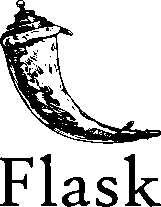
\includegraphics[width=3.5cm, height=3.5cm]{../report_MemeEcon/images/flask.png}
    \caption{Flask(\href{https://palletsprojects.com/p/flask/}{Source})}
    \label{fig:Flask}
\end{figure}

\subsection{Postman}
Postman is a platform for \ac{API} development. The Postman interface has a bunch of features that help in the building of an \ac{API} given as:
\begin{itemize}
    \item API Client: Helps to send requests within postman
    \item Automated Testing: Helps in the testing of the API
    \item Monitor: Helps to check the performance of the API
    \item Documentation: Helps to create documentation for our API
\end{itemize}
\begin{flushleft}
The \ac{API} Client allows the user to Send Requests and View response generated by the execution of the REST queries within the Postman. It also allows the user to visualize data by the use of Postman Visualizer, in our application the Postman helps to visualize the Memes and the Meme Formats. The platform also allows the user to create a test suite for their application by the use of the Collections feature, where each collection consists of multiple HTTP requests.
\end{flushleft}
\begin{figure}[H]
    \centering
    
\includegraphics[width=3.5cm, height=3.5cm]{../report_MemeEcon/images/postman.png}
    \caption{Postman(\href{https://www.postman.com/resources/media-assets/}{Source})}
    \label{fig:Postman}
\end{figure}

\section{Related Work} \label{sec:Related Work}%Rahul
% Sub-reddit approach
Reddit /r/memeEconomy, community portrays memes as a potential investment where the members can buy, sell, share, and invest in them based on their potential to become a popular meme on the website. Basically, memes and economics are combined in perfect proportion. The official currency of the subreddit is \ac{MC}.\par
\begin{flushleft}
When user create an account, they are given 10,000 \ac{MC} and also a debt of 10,000M¢ to pay back. The return on the meme investment is determined by the demand of that meme and the incentive is calculated by higher the meme charts on the subreddit, more meme coins the user earns. The Meme Economy limits the amount of \ac{MC} in the economy. It follows a risk-return trade-off pattern which is similar to crypto currencies.\par
\end{flushleft}
\begin{flushleft}
Members who create a post on /r/MemeEconomy receives \ac{MC} in the form of royalties totaling 5\% of all investments on the post. They are paid once in 24 hours after the post is released and investments after this 24 hour period will not count towards the 5\% bonus. This is a way for rewarding the creators for their work.
\end{flushleft}
% section intro and system diagram %Chris because he likes to make good looking stuff. And Mehmed too. Anant also has to be involved.

\section{Approach} \label{sec:Approach}

\subsection{Block Design} %Mehmed

Each block inside the chain has the following fields:

\begin{itemize}
  \item index - the index of the block.
  \item minerID - the id of the miner. This identification is used when distributing mining rewards.
  \item previous\_hash - the hash of the previous block inside the chain
  \item proof\_of\_work - a nonce value (magic number) which makes the hash of the block to match the difficulty pattern
  \item timestamp - an instance of time showing the creation time of the block
  \item transaction\_counter - the number of transactions inside the block
  \item transactions - a list which holds all transactions inside the block
\end{itemize}

The genesis block has "0" value on all fields and an empty list for the transactions. The hash value of the genesis block does not match any hash patterns and when validating the chain the genesis block is skipped. It should be noted that even if the block is not skipped, since all values inside the genesis block are predefined, the hash value will always be the same value and could be hard coded.

All consecutive blocks, after the genesis block, have their proper field values. The minerID field is a special field because it's value is different for each node. Each node assigns its ID to the minerID field and tries to find a nonce value with this assigned specific minerID. Also each time a new transaction is added to the memory pool of transactions, the finding nonce value process is restarted, since the transactions list is updated.


\subsection{Peer to Peer Network} %Akshay
In a blockchain peer-to-peer connection, any node connects to any other node in the network collection of nodes. The nodes in the network are connected in the form of mesh network as shown in the \ref{fig:P2P}, where each node is connected to all of its neighboring nodes and each node contains a copy of the complete blockchain. As a new node is connected to a blockchain network then all the nodes in the network are notified about the newly connected node in the network. Moreover, the newly connected node receives a copy of the complete blockchain and also receives the list of pending transactions in the blockchain. \par
\begin{flushleft}

In our application meme economy, the peer to peer concept is demonstrated by the use of the Postman as:
\begin{itemize}
    \item The core node must run on port 5000 in order to initialize the network, the port 5000 is selected specifically to prevent creation of multiple networks at the same time.
    \item Add other nodes on different port addresses.
    \item Now to show the peer to peer concept, we send a POST request using the \textbf{connect\_to\_node} method, if the request is successful we get a response showing Connection Successful on the console with status code 200.
\end{itemize}
\end{flushleft}
As the connection is successful, the newly connected node receives a copy of the blockchain and list transitions and pending transactions in the blockchain network.
\begin{figure}[H]
    \centering
    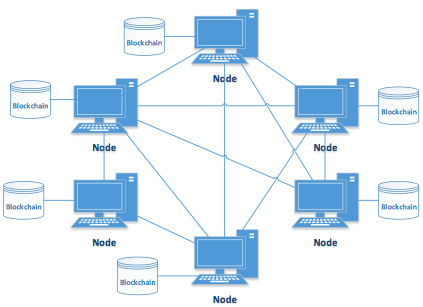
\includegraphics[width=8cm, height=5cm]{../report_MemeEcon/images/p2p.png}
    \caption{Peer-to-Peer(\href{https://www.researchgate.net/publication/320127088_Blockchain_Implementation_Quality_Challenges_A_Literature_Review/figures?lo=1&utm_source=google&utm_medium=organic}{Source})}
    \label{fig:P2P}
\end{figure}
\subsection{Transactions} %Mehmed

In the Block Design section it was discussed that each block has a list of transactions. There are 5 different kind of possible transactions:
\begin{itemize}
  \item add\_memeFormat - Used to add a new meme format to the network
  \item add\_meme - Used to add a new meme to the network
  \item add\_upvote - Used to upvote a meme inside the network
  \item sell\_ownership - Used to sell the ownership of a meme format
  \item purchase\_ownership - Used to purchase the ownership of a meme format
\end{itemize}

\subsubsection{Raw-JSON body input formats of transactions}

\begin{itemize}
\item add\_memeFormat - \{"imagePath" : "imagePathValue",\\ "name" : "nameValue"\}

\item add\_meme - \{"imagePath" : "imagePathValue",\\ "name" : "nameValue",\\ "memeFormat" : "memeFormatID"\}

\item add\_upvote - \{"imageVoteId":"memeID",\\ "upvoteID" : "upvoteID"\}

\item sell\_ownership - \{"ownershipSaleOfferID" : "ownershipSaleOfferID",\\ "memeFormat" : "memeFormatID",\\ "saleAmount" : "saleAmount"\}

\item purchase\_ownership - \{"ownershipPurchaseID" : "ownershipPurchaseID",\\ "ownershipSaleOfferID" : "ownershipSaleOfferID"\}
\end{itemize}

\subsubsection{Transaction requirements and validation}

This subsection discusses the requirements of each transaction. Once all of the requirements for a specific transaction are met, then the transaction is validated and ready to be mined in the next block.

\begin{itemize}
\item add\_memeFormat - There are not any requirements for this transaction.

\item add\_meme - Each meme to be uploaded must belong to a specific meme format. This meme format must be already mined inside a block and appended to the chain.

\item add\_upvote - The meme to be up voted must be already mined inside a block and appended to the chain. The node which up votes must have enough credits available in its wallet.

\item sell\_ownership - The meme format to be sold must be already mined inside a block and appended to the chain. The node which creates this transaction must have the ownership of the meme format to be sold.

\item purchase\_ownership - The meme format to be purchased must be already offered for a sale, mined and appended to the chain. The purchasing node must have enough credits in order to buy the meme format. The worth of the meme format is specified inside the sell\_ownership transaction.
\end{itemize}


\subsection{Mining and Consensus} %Steffen and Anant
\subsection{Wallet and Rewards} %Anant

This subsection discusses the role Wallets and Rewards play in the operation of the MemeEconomy Blockchain.

Every node has a unique and implicit wallet associated with it. Once a node mines a block or issues a transaction that is added to a block, all nodes start to internally, and independently track the state of the wallet associated with the node. Every node starts out with an initial wallet amount of 5 credits. The reason for this will be explained after a detailed explanation of rewards and credit distribution.

There are two situations in which a node is rewarded credits, either from another node, or from the system. Following are these situations:

\begin{itemize}
\item Upvote - When a meme is upvoted, a credit is deducted from the
  node that issued the upvote. This credit is then distributed in
  portions to:
  \begin{itemize}
  \item the Meme Format owner - 30\%
  \item the Meme Poster - 60\%
  \item the Meme miner - 10\%
  \end{itemize}
  In addition to this, 10\% of the upvote credits (which amounts to
  0.1 credits) are created independently and rewarded to:
  \begin{itemize}
  \item the Meme Format miner
  \item the Upvote miner
  \item every previous Upvoter from previous blocks who upvoted the
    same Meme
  \end{itemize}
\item Ownership Purchase - When a node issues a transaction to
  purchase ownership, 10\% of the sale amount is taken in excess to
  the sale amount from this node, and is shared evenly between:
  \begin{itemize}
  \item Sell transaction miner
  \item Purchase transaction miner
  \end{itemize}
  In effect, the Sell transaction miner and Purchase transaction miner
  each recieve 5\% of the sell amount.
\end{itemize}

It must be mentioned that all rewards are implicitly credited to the
respective node's wallet.

The reason for rewarding upvoters, is to incentivize upvoters who find
a meme interesting or funny. Over time (as more blocks are mined), an
upvoter is rewarded proportional to how much they contributed to the
'virality' of the meme.

There is no mechanism for a node to cancel a sell transaction. The
node is free to issue a purchase transaction for their own sell
transaction, if they see fit. In this scenario, they would lose 10\%
of the amount that they posted the ownership for sale for.

As mentioned earlier, every node is given 5 credits. This is a
necessity, since if not, no nodes have any credits to upvote, nor buy
ownership.

\subsection{Visualization} %Chris


\section{Outlook} \label{sec:Outlook} %Chris

\section{Conclusion} \label{sec:Conclusion} %Chris



\section{Template Section} \label{sec:Template}
    This template should give us a first version we can start of with. This last section should support us in writing a more coherent paper together. Therefore I put some guidelines for the writing in section~\ref{sec:Guidelines}. Also there are some example for the use of functionalities in Section~\ref{sec:Examples}. You can copy them and adapt them the way you need them. Just leave this section here for now.


    \subsection{Guidelines} \label{sec:Guidelines}
        \begin{itemize}
        \item \textbf{pushing to the repo} \\
            When you push the newest version to the repo, please leave out the files created by the compiler (besides the pdf). The report on the repo just needs the tex-file, the bib-file and maybe the most current pdf-file. Of course push the changes to the sub folders if you added images or sources.

        \item \textbf{references} \\
            For every section, subsection, figure, or table you include give it a label. Therefore everyone can refer to it later. It can be done by \textit{$\backslash$label\{marker\}}. The marker should declare the type of the object and a short (one word in the best case) name for the object. The types are "sec:" for a section, "fig:" for a figure and "tab:" for a table. You can refer to them then by \textit{$\backslash$ref\{fig:example\}}. Also you should use a $\sim$ symbol before instead of normal space to avoid line breaks there.

        \item \textbf{citations} \\
            For cititions the BibTex code for the source needs to be in the 'literature\_list.bib' file. You can usually get them pretty easily from \textit{Google Scholar}. Please safe all papers/sources you used in the "sources" folder in addition. The citation can then be made by \textit{$\backslash$cite\{antonopoulos2017mastering\}} for example. Please use the $\sim$ here too. The result then looks like this~\cite{antonopoulos2017mastering}.


        \item \textbf{abbreviations} \\
            Please use the $\backslash$ac\{...\} command to handle abbreviations. You can define them at the end of the document. Here is one example... When used the first time it automatically defines the abbreviation: \ac{AI}. For all furhter times it just prints: \ac{AI}. Also the plural is possible \acp{AI}

        \end{itemize}


    \subsection{Examples} \label{sec:Examples}

    \begin{figure}[t]
        \centering
        \subfigure[Meme Format]{
\includegraphics[width=.49\textwidth]{../memes/woman-yelling-at-cat/template.jpg}}
        \subfigure[Meme]{
\includegraphics[width=.49\textwidth]{../memes/woman-yelling-at-cat/4.jpg}}
        \caption{Example for 2 subfigures.}
        \label{fig:MemeFormat-Meme}
    \end{figure}



    \begin{figure} [t]
        \centering
        
\includegraphics[width=.3\textwidth]{../memes/drake/4.jpg}
        \caption{Example for a single figure.}
        \label{fig:drake}
    \end{figure}



    \begin{table}[t]
        \centering
        %\captionof{table}{The tasks for the different prototypes.}
        \begin{tabular}{|C{.07\textwidth}|L{.41\textwidth}|L{.41\textwidth}|}
            \hline & \textbf{SVM} & \textbf{Neural Network} \\
            \hline MR-1 & Permutation of training \& test features & Permutation of input channels (RGB channels) for
training \& test data \\
            \hline MR-2 & Permutation of order of training instances & Permutation of the convolution operation order for
training \& test data \\
            \hline MR-3 & Shifting of training \& test features by a constant (only for RBF kernel) & Normalizing the test data \\
            \hline MR-4 & Linear scaling of the test features (only for linear kernel) & Scaling the test data by a constant \\
            \hline
        \end{tabular}

        \captionof{table}{Content totally out of context, literally just as an example for a table.}
        \label{tab:relations}
    \end{table}

        \begin{center}
    \begin{lstlisting}
    # Computes the hash of the Block
    def compute_hash(self):
        # self.__dict__ -> all variables inside the Block class
        encoded_block = json.dumps(self.__dict__, sort_keys=True).encode()
        return hashlib.sha256(encoded_block).hexdigest()
    \end{lstlisting}
    \end{center}




\newpage

%-------------------References---------------------------%
\section*{Abbreviations and Acronyms}
\addcontentsline{toc}{section}{Abbreviations and Acronyms}
\begin{acronym}[Bash]
\acro{AI} {\textit{Artificial Intelligence}}
%\acro{ML} {\textit{Machine Learning}}
\acro{API}{\textit{Application Programming Interface}}
\acro{WSGI}{\textit{Web Server Gateway Interface}}
\acro{MC}{\textit{Meme Coin}}

\end{acronym}

%----------------List-of-Tables--------------------%
%Comment the following lines out if you dont have tables or figures
\listoftables
\listoffigures
\bibliographystyle{plain}
\bibliography{literature_list}
\end{document}
